\documentclass[12pt]{article}
\usepackage{graphicx}
\usepackage{amsmath}
\usepackage{mathtools}
\usepackage{gensymb}

\newcommand{\mydet}[1]{\ensuremath{\begin{vmatrix}#1\end{vmatrix}}}
\providecommand{\brak}[1]{\ensuremath{\left(#1\right)}}
\providecommand{\norm}[1]{\left\lVert#1\right\rVert}
\newcommand{\solution}{\noindent \textbf{Solution: }}
\newcommand{\myvec}[1]{\ensuremath{\begin{pmatrix}#1\end{pmatrix}}}
\let\vec\mathbf
\def\inputGnumericTable{}
\usepackage{color}                                            %%
    \usepackage{array}                                            %%
    \usepackage{longtable}                                        %%
    \usepackage{calc}                                             %%
    \usepackage{multirow}                                         %%
    \usepackage{hhline}                                           %%
    \usepackage{ifthen}
\usepackage{array}
\usepackage{amsmath}   % for having text in math mode
\usepackage{listings}
\lstset{
language=tex,
frame=single, 
breaklines=true
}
\begin{document}
\begin{center}
\textbf\large{CLASS-9\\CHAPTER-10 \\ CIRCLES}

\end{center}
\section*{Excercise 10.5}

Q1. In Figure 1. $\vec{A},\vec{B},\vec{C}$ are the three points with centre $\vec{O}$ such that $\angle$ BOC=30\degree and $\angle$ AOB=60\degree. If $\vec{D}$ is a point on the circle other than the arc ABC, find $\angle$ADC
\section*{\large Solution}
\begin{figure}[h!]
\centering
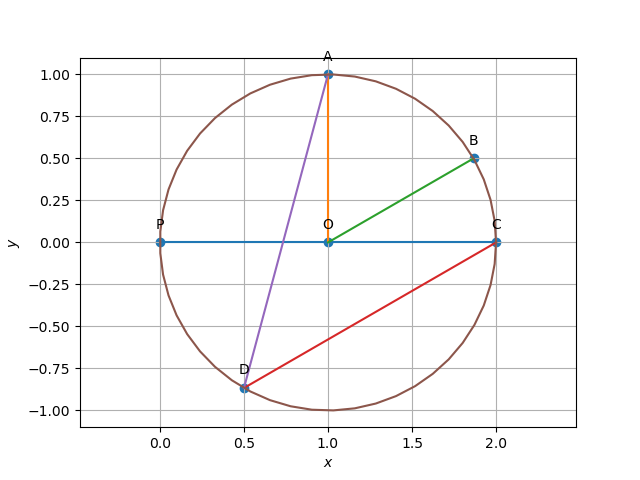
\includegraphics[width=\columnwidth]{figs/circle2.png}
\caption{}
\label{fig:Fig1}
\end{figure}
\section*{\large Construction}

\begin{table}[ht!]
%%%%%%%%%%%%%%%%%%%%%%%%%%%%%%%%%%%%%%%%%%%%%%%%%%%%%%%%%%%%%%%%%%%%%%
%%                                                                  %%
%%  This is the header of a LaTeX2e file exported from Gnumeric.    %%
%%                                                                  %%
%%  This file can be compiled as it stands or included in another   %%
%%  LaTeX document. The table is based on the longtable package so  %%
%%  the longtable options (headers, footers...) can be set in the   %%
%%  preamble section below (see PRAMBLE).                           %%
%%                                                                  %%
%%  To include the file in another, the following two lines must be %%
%%  in the including file:                                          %%
%%        \def\inputGnumericTable{}                                 %%
%%  at the beginning of the file and:                               %%
%%        \input{name-of-this-file.tex}                             %%
%%  where the table is to be placed. Note also that the including   %%
%%  file must use the following packages for the table to be        %%
%%  rendered correctly:                                             %%
%%    \usepackage[latin1]{inputenc}                                 %%
%%    \usepackage{color}                                            %%
%%    \usepackage{array}                                            %%
%%    \usepackage{longtable}                                        %%
%%    \usepackage{calc}                                             %%
%%    \usepackage{multirow}                                         %%
%%    \usepackage{hhline}                                           %%
%%    \usepackage{ifthen}                                           %%
%%  optionally (for landscape tables embedded in another document): %%
%%    \usepackage{lscape}                                           %%
%%                                                                  %%
%%%%%%%%%%%%%%%%%%%%%%%%%%%%%%%%%%%%%%%%%%%%%%%%%%%%%%%%%%%%%%%%%%%%%



%%  This section checks if we are begin input into another file or  %%
%%  the file will be compiled alone. First use a macro taken from   %%
%%  the TeXbook ex 7.7 (suggestion of Han-Wen Nienhuys).            %%
\def\ifundefined#1{\expandafter\ifx\csname#1\endcsname\relax}


%%  Check for the \def token for inputed files. If it is not        %%
%%  defined, the file will be processed as a standalone and the     %%
%%  preamble will be used.                                          %%
\ifundefined{inputGnumericTable}

%%  We must be able to close or not the document at the end.        %%
	\def\gnumericTableEnd{\end{document}}


%%%%%%%%%%%%%%%%%%%%%%%%%%%%%%%%%%%%%%%%%%%%%%%%%%%%%%%%%%%%%%%%%%%%%%
%%                                                                  %%
%%  This is the PREAMBLE. Change these values to get the right      %%
%%  paper size and other niceties.                                  %%
%%                                                                  %%
%%%%%%%%%%%%%%%%%%%%%%%%%%%%%%%%%%%%%%%%%%%%%%%%%%%%%%%%%%%%%%%%%%%%%%

	\documentclass[12pt%
			  %,landscape%
                    ]{report}
       \usepackage[latin1]{inputenc}
       \usepackage{fullpage}
       \usepackage{color}
       \usepackage{array}
       \usepackage{longtable}
       \usepackage{calc}
       \usepackage{multirow}
       \usepackage{hhline}
       \usepackage{ifthen}
       \usepackage{gensymb}
       \usepackage{graphicx}
\usepackage{amsmath}
\usepackage{mathtools}
\newcommand{\mydet}[1]{\ensuremath{\begin{vmatrix}#1\end{vmatrix}}}
\providecommand{\brak}[1]{\ensuremath{\left(#1\right)}}
\providecommand{\norm}[1]{\left\lVert#1\right\rVert}
\newcommand{\solution}{\noindent \textbf{Solution: }}
\newcommand{\myvec}[1]{\ensuremath{\begin{pmatrix}#1\end{pmatrix}}}
\let\vec\mathbf
	\begin{document}


%%  End of the preamble for the standalone. The next section is for %%
%%  documents which are included into other LaTeX2e files.          %%
\else

%%  We are not a stand alone document. For a regular able, we will %%
%%  have no preamble and only define the closing to mean nothing.   %%
    \def\gnumericTableEnd{}

%%  If we want landscape mode in an embedded document, comment out  %%
%%  the line above and uncomment the two below. The table will      %%
%%  begin on a new page and run in landscape mode.                  %%
%       \def\gnumericTableEnd{\end{landscape}}
%       \begin{landscape}


%%  End of the else clause for this file being \input.              %%
\fi

%%%%%%%%%%%%%%%%%%%%%%%%%%%%%%%%%%%%%%%%%%%%%%%%%%%%%%%%%%%%%%%%%%%%%%
%%                                                                  %%
%%  The rest is the gnumeric table, except for the closing          %%
%%  statement. Changes below will alter the table's appearance.     %%
%%                                                                  %%
%%%%%%%%%%%%%%%%%%%%%%%%%%%%%%%%%%%%%%%%%%%%%%%%%%%%%%%%%%%%%%%%%%%%%%
\providecommand{\gnumericmathit}[1]{#1} 
%%  Uncomment the next line if you would like your numbers to be in %%
%%  italics if they are italizised in the gnumeric table.           %%
%\renewcommand{\gnumericmathit}[1]{\mathit{#1}}
\providecommand{\gnumericPB}[1]%
{\let\gnumericTemp=\\#1\let\\=\gnumericTemp\hspace{0pt}}
 \ifundefined{gnumericTableWidthDefined}
        \newlength{\gnumericTableWidth}
        \newlength{\gnumericTableWidthComplete}
        \newlength{\gnumericMultiRowLength}
        \global\def\gnumericTableWidthDefined{}
 \fi
%% The following setting protects this code from babel shorthands.  %%
 \ifthenelse{\isundefined{\languageshorthands}}{}{\languageshorthands{english}}
%%  The default table format retains the relative column widths of  %%
%%  gnumeric. They can easily be changed to c, r or l. In that case %%
%%  you may want to comment out the next line and uncomment the one %%
%%  thereafter                                                      %%
\providecommand\gnumbox{\makebox[0pt]}
%%\providecommand\gnumbox[1][]{\makebox}

%% to adjust positions in multirow situations                       %%
\setlength{\bigstrutjot}{\jot}
\setlength{\extrarowheight}{\doublerulesep}

%%  The \setlongtables command keeps column widths the same across  %%
%%  pages. Simply comment out next line for varying column widths.  %%
\setlongtables

\setlength\gnumericTableWidth{%
	40pt+%
	35pt+%
	210pt+%
0pt}
\def\gumericNumCols{3}
\setlength\gnumericTableWidthComplete{\gnumericTableWidth+%
         \tabcolsep*\gumericNumCols*2+\arrayrulewidth*\gumericNumCols}
\ifthenelse{\lengthtest{\gnumericTableWidthComplete > \linewidth}}%
         {\def\gnumericScale{\ratio{\linewidth-%
                        \tabcolsep*\gumericNumCols*2-%
                        \arrayrulewidth*\gumericNumCols}%
{\gnumericTableWidth}}}%
{\def\gnumericScale{1}}

%%%%%%%%%%%%%%%%%%%%%%%%%%%%%%%%%%%%%%%%%%%%%%%%%%%%%%%%%%%%%%%%%%%%%%
%%                                                                  %%
%% The following are the widths of the various columns. We are      %%
%% defining them here because then they are easier to change.       %%
%% Depending on the cell formats we may use them more than once.    %%
%%                                                                  %%
%%%%%%%%%%%%%%%%%%%%%%%%%%%%%%%%%%%%%%%%%%%%%%%%%%%%%%%%%%%%%%%%%%%%%%

\ifthenelse{\isundefined{\gnumericColA}}{\newlength{\gnumericColA}}{}\settowidth{\gnumericColA}{\begin{tabular}{@{}p{40pt*\gnumericScale}@{}}x\end{tabular}}
\ifthenelse{\isundefined{\gnumericColB}}{\newlength{\gnumericColB}}{}\settowidth{\gnumericColB}{\begin{tabular}{@{}p{35pt*\gnumericScale}@{}}x\end{tabular}}
\ifthenelse{\isundefined{\gnumericColC}}{\newlength{\gnumericColC}}{}\settowidth{\gnumericColC}{\begin{tabular}{@{}p{210pt*\gnumericScale}@{}}x\end{tabular}}

\begin{longtable}[c]{%
	b{\gnumericColA}%
	b{\gnumericColB}%
	b{\gnumericColC}%
	}

%%%%%%%%%%%%%%%%%%%%%%%%%%%%%%%%%%%%%%%%%%%%%%%%%%%%%%%%%%%%%%%%%%%%%%
%%  The longtable options. (Caption, headers... see Goosens, p.124) %%
%	\caption{The Table Caption.}             \\	%
% \hline	% Across the top of the table.
%%  The rest of these options are table rows which are placed on    %%
%%  the first, last or every page. Use \multicolumn if you want.    %%

%%  Header for the first page.                                      %%
%	\multicolumn{3}{c}{The First Header} \\ \hline 
%	\multicolumn{1}{c}{colTag}	%Column 1
%	&\multicolumn{1}{c}{colTag}	%Column 2
%	&\multicolumn{1}{c}{colTag}	\\ \hline %Last column
%	\endfirsthead

%%  The running header definition.                                  %%
%	\hline
%	\multicolumn{3}{l}{\ldots\small\slshape continued} \\ \hline
%	\multicolumn{1}{c}{colTag}	%Column 1
%	&\multicolumn{1}{c}{colTag}	%Column 2
%	&\multicolumn{1}{c}{colTag}	\\ \hline %Last column
%	\endhead

%%  The running footer definition.                                  %%
%	\hline
%	\multicolumn{3}{r}{\small\slshape continued\ldots} \\
%	\endfoot

%%  The ending footer definition.                                   %%
%	\multicolumn{3}{c}{That's all folks} \\ \hline 
%	\endlastfoot
%%%%%%%%%%%%%%%%%%%%%%%%%%%%%%%%%%%%%%%%%%%%%%%%%%%%%%%%%%%%%%%%%%%%%%

\hhline{|-|-|-}
	 \multicolumn{1}{|p{\gnumericColA}|}%
	{\gnumericPB{\raggedright}\gnumbox[l]{\textbf{Symbol}}}
	&\multicolumn{1}{p{\gnumericColB}|}%
	{\gnumericPB{\raggedright}\gnumbox[l]{\textbf{Values}}}
	&\multicolumn{1}{p{\gnumericColC}|}%
	{\gnumericPB{\raggedright}\gnumbox[l]{\textbf{Description}}}
\\
\hhline{|---|}
	 \multicolumn{1}{|p{\gnumericColA}|}%
	{\gnumericPB{\raggedright}\gnumbox[l]{$\vec{A}$}}
	&\multicolumn{1}{p{\gnumericColB}|}%
	{\gnumericPB{\raggedright}\gnumbox[l]{$\vec{0}$}}
	&\multicolumn{1}{p{\gnumericColC}|}%
	{\gnumericPB{\raggedright}\gnumbox[l]{Center of circle 1}}
\\
\hhline{|---|}
	 \multicolumn{1}{|p{\gnumericColA}|}%
	{\gnumericPB{\raggedright}\gnumbox[l]{$r_1$}}
	&\multicolumn{1}{p{\gnumericColB}|}%
	{\gnumericPB{\raggedright}\gnumbox[l]{3 units}}
	&\multicolumn{1}{p{\gnumericColC}|}%
	{\gnumericPB{\raggedright}\gnumbox[l]{Radius of the circle 1 }}
\\
\hhline{|---|}
	 \multicolumn{1}{|p{\gnumericColA}|}%
	{\gnumericPB{\raggedright}\gnumbox[l]{$\vec{B}$}}
	&\multicolumn{1}{p{\gnumericColB}|}%
	{\gnumericPB{\raggedright}\gnumbox[l]{\myvec{4\\0}}}
	&\multicolumn{1}{p{\gnumericColC}|}%
	{\gnumericPB{\raggedright}\gnumbox[l]{Center of circle 2}}
\\
\hhline{|---|}
	 \multicolumn{1}{|p{\gnumericColA}|}%
	{\gnumericPB{\raggedright}\gnumbox[l]{$r_2$}}
	&\multicolumn{1}{p{\gnumericColB}|}%
	{\gnumericPB{\raggedright}\gnumbox[l]{2 units}}
	&\multicolumn{1}{p{\gnumericColC}|}%
	{\gnumericPB{\raggedright}\gnumbox[l]{Radius of circle 2}}
\\
\hhline{|---|}
	 \multicolumn{1}{|p{\gnumericColA}|}%
	{\gnumericPB{\raggedright}\gnumbox[l]{$\vec{e}_1$}}
	&\multicolumn{1}{p{\gnumericColB}|}%
	{\gnumericPB{\raggedright}\gnumbox[l]{\myvec{1\\0}}}
	&\multicolumn{1}{p{\gnumericColC}|}%
	{\gnumericPB{\raggedright}\gnumbox[l]{Standard basis vector 1}}
\\
\hhline{|---|}
\multicolumn{1}{|p{\gnumericColA}|}%
	{\gnumericPB{\raggedright}\gnumbox[l]{$\vec{e}_2$}}
	&\multicolumn{1}{p{\gnumericColB}|}%
	{\gnumericPB{\raggedright}\gnumbox[l]{\myvec{0\\1}}}
	&\multicolumn{1}{p{\gnumericColC}|}%
	{\gnumericPB{\raggedright}\gnumbox[l]{Standard basis vector 2}}
	\\
\hhline{|---|}
\end{longtable}

\ifthenelse{\isundefined{\languageshorthands}}{}{\languageshorthands{\languagename}}
\gnumericTableEnd%t

\caption{}
\label{Table-1} 
\end{table}


\section*{\large Assumptions}
\begin{enumerate}
	\item Let $\vec{P}$ be a point on the circle such that by expandig OC upto $\vec{P}$ we get diameter POC.
\item To find $\angle$ADC let the circle be unit circle and diameter POC on x axis.
\item Take three points $\vec{C},\vec{A},\vec{D}$ and $\alpha$,$\beta$,$\gamma$ be three angles made by the points $\vec{C},\vec{A},\vec{D}$ with respect to diameter POC.
\end{enumerate}
From the Figure \ref{fig:Fig1}:
\begin{align}
\alpha = {\angle POC}= 180\degree, 
\beta= {\angle POA} = 90\degree,
\gamma = {\angle POD}=300\degree
\end{align}
\section*{Verification:}
From assumptions the vector points $\vec{C},\vec{A},\vec{D}$ be
\begin{align}
	\vec{C} = \myvec{\cos\alpha\\\sin\alpha},
	\vec{A} = \myvec{\cos\beta\\\sin\beta},
	\vec{D} = \myvec{\cos\gamma\\\sin\gamma}
\end{align}
Let AC be the chord that subtends angles at the center $\vec{O}$ and at point $\vec{D}$. The cosine of the angle subtended at point $\vec{D}$ is given by
\begin{align}
	\cos(\angle ADC) = \frac{\vec{(A-D)^\top(C-D)}}{\norm{\vec{A-D}}\norm{\vec{C-D}}}
	\label{eq:3}
\end{align}
Where
 \begin{align}
	 \vec{A-D}& = \myvec{\cos\beta - \cos\gamma\\\sin\beta - \sin\gamma},
	 \vec{C-D} = \myvec{\cos\alpha - \cos\gamma\\\sin\alpha - \sin\gamma}\\
	 \label{eq:5} \vec{(A-D)^\top(C-D)}&= 4\sin\frac{\alpha-\gamma}2\sin\frac{\beta-\gamma}2\cos\frac{\alpha-\beta}2\\
	 \norm{\vec{A-D}}\norm{\vec{C-D}}& = 4 \sin\frac{\alpha-\gamma}2\sin\frac{\beta-\gamma}2
	\label{eq:6}
\end{align}
Substituting \eqref{eq:5} and \eqref{eq:6} in \eqref{eq:3},
\begin{align}
	\cos(\angle ADC) &= \frac{4\sin\frac{\alpha-\gamma}{2}\sin\frac{\beta-\gamma}{2}\cos\frac{\alpha-\beta}{2}}{4 \sin\frac{\alpha-\gamma}2\sin\frac{\beta-\gamma}2}\\
	\cos(\angle ADC) &= \cos\frac{\alpha-\beta}{2}
	\label{eq:11}
\end{align}
By substituting $\alpha$ and $\beta$ values in \eqref{eq:11}
\begin{align}
\angle ADC = \frac{\alpha-\beta}{2}=\frac{(180\degree - 90\degree )}{2}=45\degree
\end{align}



\end{document}
